\documentclass[12pt,a4paper]{article}

\usepackage[a4paper,margin=1in]{geometry}
\usepackage{amsmath}
\usepackage{amssymb}
\usepackage{fancyhdr}
\usepackage{tikz}
\usepackage{array}
\usepackage{enumitem}
\usepackage{xcolor}
\usepackage{titlesec}

\usetikzlibrary{calc,arrows.meta,positioning}

% ---------- Footer ----------
\pagestyle{fancy}
\fancyhf{}
\renewcommand{\headrulewidth}{0pt}
\renewcommand{\footrulewidth}{0pt}
\fancyfoot[C]{\footnotesize\textcolor{gray!70}{The Student Hub $\cdot$ Kerwin Springer $\cdot$ Worked CSEC Maths Solutions}}
\fancyfoot[R]{\footnotesize\textcolor{gray!70}{\thepage}}

\fancypagestyle{plain}{%
  \fancyhf{}%
  \renewcommand{\headrulewidth}{0pt}%
  \fancyfoot[C]{\footnotesize\textcolor{gray!70}{The Student Hub $\cdot$ Kerwin Springer $\cdot$ Worked CSEC Maths Solutions}}%
}

% ---------- Question heading style ----------
\newcommand{\qhead}[1]{\vspace{0.6em}\noindent\textbf{\large #1}\par\vspace{0.3em}}
\newcommand{\subhead}[1]{\vspace{0.3em}\noindent\textbf{#1}\par}
\newcommand{\qmarks}[1]{\hfill\textit{(#1)}}

\setlength{\parindent}{0pt}
\setlength{\parskip}{0.5em}

\titleformat{\section}{\normalfont\Large\bfseries}{\thesection}{1em}{}
\titlespacing*{\section}{0pt}{1em}{0.6em}

\begin{document}

% ---------- Cover Page ----------
\thispagestyle{plain}
\begin{center}
\vspace*{2cm}
{\Huge\bfseries CSEC Mathematics}\\[1em]
{\LARGE May/June 2026 -- Paper 2}\\[1em]
{\LARGE Worked Solutions}\\[2em]
{\normalsize\itshape Reviewed and published by Kerwin Springer at The Student Hub}
\end{center}
\vfill
\newpage

% ---------- Section I ----------
\begin{center}
{\large\bfseries SECTION I}\\[0.4em]
Answer ALL questions.\\
All working must be clearly shown.
\end{center}

% ==========================================================
\qhead{1. (a) (i) Write the following numbers correct to 1 significant figure.}

$0.367$
\[ 0.367 \approx 0.4 \text{ to 1 sf} \]

$3.94$
\[ 3.94 \approx 4 \text{ to 1 sf} \]
\qmarks{2 marks}

\subhead{(ii) Hence, estimate the integer value of $\dfrac{\sqrt{1000}\times 0.367}{3.94}$.}
\begin{align*}
\frac{\sqrt{1000}\times 0.367}{3.94} &\approx \frac{\sqrt{1000}\times 0.4}{4} \\
&= \sqrt{100} \\
&= 10
\end{align*}
\qmarks{1 mark}

\subhead{(b) Aiden, Brooke and Caden share berries in the ratio $3:2:5$. Aiden receives 12 more berries than Brooke. Calculate the TOTAL number of berries shared.}

Difference:
\begin{align*}
\text{Aiden} - \text{Brooke} &= 3\text{ parts} - 2\text{ parts} \\
&= 1\text{ part} \\
1\text{ part} &= 12
\end{align*}
\begin{align*}
\text{Total parts} &= 3+2+5 = 10\text{ parts} \\
\text{Total berries} &= 10\times 12 = 120 \text{ berries}
\end{align*}
\qmarks{2 marks}

\subhead{(c) In a sale, all prices are reduced by 15\%.}

\textit{(i) Blake buys a book which has an original price of \$16.40. Calculate how much he pays.}
\begin{align*}
\text{Sale price} &= 85\% \text{ of original price} \\
&= 0.85 \times 16.40 \\
&= \$13.94
\end{align*}
\qmarks{2 marks}

\textit{(ii) Jude pays \$27.20 for a toy. Calculate the original price of the toy.}
\begin{align*}
85\% &= 27.20 \\
1\% &= \frac{27.20}{85} \\
\text{Original price (100\%)} &= \frac{27.20}{85}\times 100 \\
&= \$32.00
\end{align*}
\qmarks{2 marks}

\hfill\textit{Total 9 marks}

\newpage
% ==========================================================
\qhead{2. (a) Given that $A = \dfrac{p^2 - q}{2r}$,}

\subhead{(i) find the value of $A$ when $p = 2$, $q = -1$ and $r = 1$.}
\begin{align*}
A &= \frac{p^2 - q}{2r} \\
&= \frac{(2)^2 - (-1)}{2\times(1)} \\
&= \frac{4+1}{2} \\
&= 2.5
\end{align*}
\qmarks{1 mark}

\subhead{(ii) Express $q$ in terms of $A$, $p$ and $r$.}
\begin{align*}
A &= \frac{p^2 - q}{2r} \\
2Ar &= p^2 - q \\
q &= p^2 - 2Ar
\end{align*}
\qmarks{2 marks}

\subhead{(b) In triangle EFG, $EG = (2x+3)$ cm and the perpendicular height from $F$ to $EG$ is $(x+5)$ cm. Given that the area of triangle EFG $= 50$ cm$^2$,}

\begin{center}
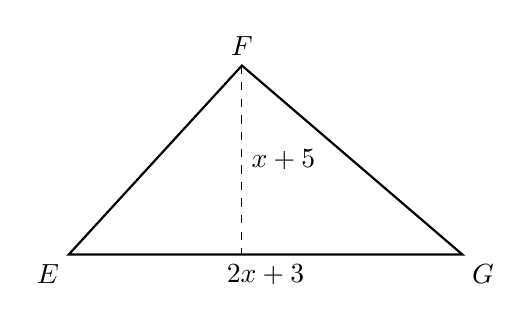
\begin{tikzpicture}[scale=1]
\coordinate (E) at (0,0);
\coordinate (G) at (5,0);
\coordinate (F) at (2.2,2.4);
\draw[thick] (E)--(G)--(F)--cycle;
\node[below left] at (E) {$E$};
\node[below right] at (G) {$G$};
\node[above] at (F) {$F$};
\node[below] at (2.5,0) {$2x+3$};
\draw[dashed] (F)--(2.2,0);
\node[right] at (2.2,1.2) {$x+5$};
\end{tikzpicture}
\end{center}

\subhead{(i) Show that $2x^2 + 13x - 85 = 0$.}
\begin{align*}
\text{Area} &= \tfrac{1}{2}\times \text{base}\times\text{height} \\
50 &= \tfrac{1}{2}(2x+3)(x+5) \\
100 &= (2x+3)(x+5) \\
100 &= 2x^2 + 10x + 3x + 15 \\
100 &= 2x^2 + 13x + 15 \\
2x^2 + 13x - 85 &= 0
\end{align*}
\qmarks{3 marks}

\subhead{(ii) Find the value of $x$, correct to 2 decimal places.}

Using the Quadratic Formula with $a = 2$, $b = 13$, $c = -85$:
\begin{align*}
x &= \frac{-b \pm \sqrt{b^2 - 4ac}}{2a} \\
&= \frac{-13 \pm \sqrt{13^2 - 4(2)(-85)}}{2(2)} \\
&= \frac{-13 \pm \sqrt{849}}{4}
\end{align*}
\[ x = 4.03 \quad \text{or} \quad x = -10.53 \]
Since length must be positive, $x = 4.03$.
\qmarks{3 marks}

\hfill\textit{Total 9 marks}

\newpage
% ==========================================================
\qhead{3. In the diagram, JKL is a straight line and JMK is a right-angled triangle. The line segment JM is parallel to KQ, $JK = 12$ cm and $MK = 8$ cm.}

\begin{center}
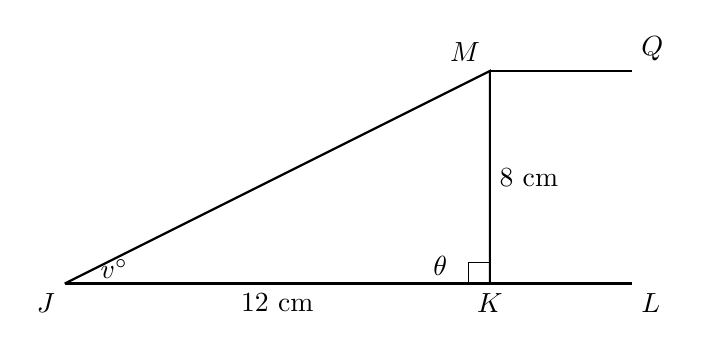
\begin{tikzpicture}[scale=0.9]
\coordinate (J) at (0,0);
\coordinate (K) at (6,0);
\coordinate (L) at (8,0);
\coordinate (M) at (6,3);
\coordinate (Q) at (8,3);
\draw[thick] (J)--(L);
\draw[thick] (J)--(M)--(K);
\draw[thick] (M)--(Q);
\draw (5.7,0) rectangle (6,0.3);
\node[below left] at (J) {$J$};
\node[below] at (K) {$K$};
\node[below right] at (L) {$L$};
\node[above left] at (M) {$M$};
\node[above right] at (Q) {$Q$};
\node[below] at (3,0) {$12$ cm};
\node[right] at (6,1.5) {$8$ cm};
\node at (0.7,0.2) {$v^{\circ}$};
\node at (5.3,0.25) {$\theta$};
\end{tikzpicture}
\end{center}

\subhead{(a) Determine}

\textit{(i) $\sin v^{\circ}$.}
\begin{align*}
\sin v^{\circ} &= \frac{\text{opposite}}{\text{hypotenuse}} = \frac{MK}{JK} \\
&= \frac{8}{12} = \frac{2}{3}
\end{align*}
\qmarks{1 mark}

\textit{(ii) The length of $JM$.}
\begin{align*}
JM^2 + MK^2 &= JK^2 \\
JM^2 + (8)^2 &= 12^2 \\
JM^2 &= 144 - 64 = 80 \\
JM &= \sqrt{80} = 8.94 \text{ cm to 3 sf}
\end{align*}
\qmarks{2 marks}

\textit{(iii) $\angle MKL$.}
\begin{align*}
\cos\theta &= \frac{\text{adj}}{\text{hyp}} = \frac{8}{12} \\
\theta &= \cos^{-1}\!\left(\frac{8}{12}\right) = 48.2^{\circ}
\end{align*}
\[ \angle MKL = 180^{\circ} - 48.2^{\circ} = 131.8^{\circ} \]
\qmarks{2 marks}

\subhead{(b) Construct a trapezium WXYZ, with $WX = 9$ cm, $XY = 5$ cm, $YZ = 3$ cm, $\angle WXY = 60^{\circ}$ and $WX \parallel YZ$.}

\begin{center}
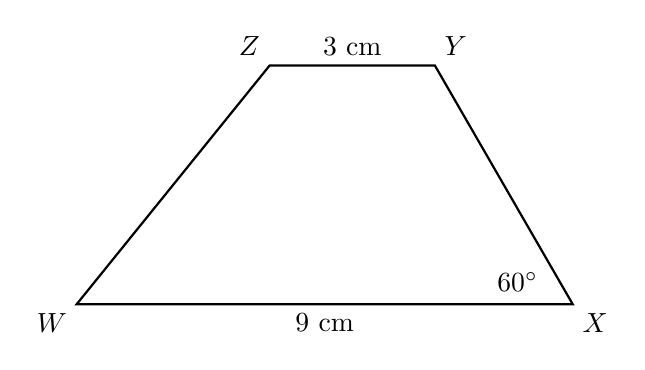
\begin{tikzpicture}[scale=0.7]
\coordinate (W) at (0,0);
\coordinate (X) at (9,0);
\coordinate (Y) at (9-5*0.5, 5*0.866);
\coordinate (Z) at ($(Y) - (3,0)$);
\draw[thick] (W)--(X)--(Y)--(Z)--cycle;
\node[below left] at (W) {$W$};
\node[below right] at (X) {$X$};
\node[above right] at (Y) {$Y$};
\node[above left] at (Z) {$Z$};
\node[below] at (4.5,0) {$9$ cm};
\node[above] at ($(Y)!0.5!(Z)$) {$3$ cm};
\node at (8,0.4) {$60^{\circ}$};
\end{tikzpicture}
\end{center}
\qmarks{4 marks}

\hfill\textit{Total 9 marks}

\newpage
% ==========================================================
\qhead{4. (a) The coordinates of $A$ and $B$ are $(-3,-4)$ and $(2,6)$ respectively. For the line segment $AB$, determine:}

\subhead{(i) Midpoint, $M$.}
\begin{align*}
M &= \left( \frac{x_1 + x_2}{2},\; \frac{y_1 + y_2}{2} \right) \\
&= \left( \frac{-3 + 2}{2},\; \frac{-4 + 6}{2} \right) \\
&= \left( -\tfrac{1}{2},\; 1 \right)
\end{align*}
\qmarks{2 marks}

\subhead{(ii) Gradient, $m$.}
\begin{align*}
m &= \frac{y_2 - y_1}{x_2 - x_1} \\
&= \frac{6 - (-4)}{2 - (-3)} \\
&= \frac{10}{5} = 2
\end{align*}
\qmarks{2 marks}

\subhead{(iii) Equation of its perpendicular bisector.}

Gradient of $AB = 2$, so gradient of perpendicular bisector $= -\tfrac{1}{2}$.

Using midpoint $\left( -\tfrac{1}{2}, 1 \right)$:
\begin{align*}
y - y_1 &= m(x - x_1) \\
y - 1 &= -\tfrac{1}{2}\left(x + \tfrac{1}{2}\right) \\
y &= -\tfrac{1}{2}x + \tfrac{3}{4}
\end{align*}
\qmarks{3 marks}

\subhead{(b) Another point $Z$ has coordinates $(-5,-8)$. Show that points $A$, $B$ and $Z$ are collinear.}

$A = (-3,-4)$, $B = (2,6)$, $Z = (-5,-8)$.

Equation of $AB$:
\begin{align*}
y - y_1 &= m(x - x_1) \\
y - 6 &= 2(x - 2) \\
y &= 2x - 4 + 6 \\
y &= 2x + 2
\end{align*}

Substitute $Z(-5,-8)$:
\begin{align*}
-8 &= 2(-5) + 2 \\
-8 &= -10 + 2 \\
-8 &= -8 \quad \text{Q.E.D.}
\end{align*}
Therefore $A$, $B$ and $Z$ are collinear.

\hfill\textit{Total 9 marks}

\newpage
% ==========================================================
\qhead{5. (a) The frequency table below shows the number of goals scored in a series of football matches.}

\begin{center}
\begin{tabular}{|l|c|c|c|c|c|c|}
\hline
Number of Goals scored & 0 & 1 & 2 & 3 & 4 & 5 \\ \hline
Number of Matches & 3 & 10 & $k$ & 15 & 4 & 3 \\ \hline
\end{tabular}
\end{center}

If the mean number of goals is $2.2$, determine $k$.
\begin{align*}
\text{Mean} &= \frac{\Sigma fx}{\Sigma f} \\
2.2 &= \frac{0(3) + 1(10) + 2k + 3(15) + 4(4) + 5(3)}{3 + 10 + k + 15 + 4 + 3} \\
2.2 &= \frac{86 + 2k}{35 + k} \\
2.2(35 + k) &= 86 + 2k \\
77 + 2.2k &= 86 + 2k \\
0.2k &= 9 \\
k &= 45
\end{align*}
\qmarks{3 marks}

\subhead{(b) Teacher Joy recorded the time taken for the 60 students in her Math Club to complete a 12-piece puzzle. The cumulative frequency graph shows information on the time taken.}

\begin{center}
\fbox{\parbox{0.7\textwidth}{\centering\itshape [Cumulative frequency curve --- see original paper]}}
\end{center}

\subhead{(i) Probability that a student chosen at random takes at least 42 seconds.}

From the curve, cumulative frequency at 42 seconds is $15$.
\begin{align*}
\text{Number taking at least 42 s} &= 60 - 15 = 45 \\
P &= \frac{45}{60} = 0.75 \text{ or } 75\%
\end{align*}
\qmarks{2 marks}

\subhead{(ii) Use the curve to determine the semi-interquartile range.}
\begin{align*}
Q_1 &= \frac{n+1}{4} = \frac{60+1}{4} \\
Q_1 &\text{ is the } 15.25\text{th value} \approx 42\text{ s (from graph)}
\end{align*}
\begin{align*}
Q_3 &= \frac{3}{4}(n+1) = \frac{3}{4}(61) \\
Q_3 &\text{ is the } 45.75\text{th value} \approx 64\text{ s (from graph)}
\end{align*}
\begin{align*}
\text{Semi-interquartile range} &= \frac{Q_3 - Q_1}{2} \\
&= \frac{64 - 42}{2} = 11 \text{ s}
\end{align*}
\qmarks{2 marks}

\subhead{(iii) Complete the table below.}

\begin{center}
\begin{tabular}{|l|c|c|c|}
\hline
Time Taken (s) & Number of Students ($f$) & Midpoint ($x$) & $fx$ \\ \hline
21--40 & 13 & 30.5 & 396.5 \\ \hline
41--60 & 28 & 50.5 & 1414 \\ \hline
61--80 & 16 & 70.5 & 1128 \\ \hline
81--100 & 3 & 90.5 & 271.5 \\ \hline
\end{tabular}
\end{center}

2nd interval: $41 - 13 = 28$. Total $= 57$, therefore $57 - (28+13) = 16$. Then $28\times 50.5 = 1414$ and $16\times 70.5 = 1128$.
\qmarks{2 marks}

\hfill\textit{Total 9 marks}

\newpage
% ==========================================================
\qhead{6. (a) A recipe for 20 bite-size cookies uses 175 g flour, 125 g butter and 75 g sugar.}

\subhead{(i) Ratio of flour to butter to sugar, in simplest form.}
\[ 175 : 125 : 75 \quad=\quad 7 : 5 : 3 \]

\subhead{(ii) Amount of flour, butter and sugar needed for 52 cookies.}
\begin{align*}
\text{Scale factor} &= \frac{52}{20} = 2.6 \\
\text{Flour} &= 175\times 2.6 = 455\text{ g} \\
\text{Butter} &= 125\times 2.6 = 325\text{ g} \\
\text{Sugar} &= 75\times 2.6 = 195\text{ g}
\end{align*}
\qmarks{3 marks}

\subhead{(b) Cookies are made and sold in packs of 12. A bag of flour contains 12.65 kg.}

\textit{One bag of flour makes a MAXIMUM of \underline{\hspace{2em}} packs of cookies.}\\
\textit{The amount of flour left over is \underline{\hspace{2em}} g.}
\begin{align*}
\text{Flour for 12 cookies} &= \frac{12}{20}\times 175 = 105\text{ g} \\
12.65\text{ kg} &= 12650\text{ g} \\
\text{Max number of packs} &= 12650 \div 105 \\
&= 120 \text{ remainder } 50
\end{align*}

One bag of flour makes a MAXIMUM of \textbf{120} packs of cookies.\\
The amount of flour left over is \textbf{50} g.
\qmarks{4 marks}

\hfill\textit{Total 9 marks}

\newpage
% ==========================================================
\qhead{7. (a) The diagram below shows part of a number chart. The numbers on the chart follow various patterns. Study the patterns and answer the questions that follow.}

\begin{center}
\begin{tabular}{|c|c|c|c|c|}
\hline
\multicolumn{2}{|c|}{} & \multicolumn{3}{c|}{Column} \\ \cline{3-5}
\multicolumn{2}{|c|}{} & 1 & 2 & 3 \\ \hline
 & 1 & 7  & 9  & 11 \\ \cline{2-5}
 & 2 & 14 & 16 & 18 \\ \cline{2-5}
Row & 3 & 21 & 23 & 25 \\ \cline{2-5}
 & 4 & 28 & 30 & 32 \\ \cline{2-5}
 & 5 & 35 & 37 & 39 \\ \cline{2-5}
 & 6 & 42 & 44 & 46 \\ \hline
\end{tabular}
\end{center}

\subhead{(i) What number should be placed in Column 1, Row 9?}

In Column 1, the numbers are multiples of 7.
\begin{align*}
\text{Row 9, Column 1} &= 7\times 9 = 63
\end{align*}
\qmarks{1 mark}

\subhead{(ii) The following diagram represents a given row from the chart.}

\begin{center}
\begin{tabular}{|c|c|c|c|}
\hline
& \multicolumn{3}{c|}{Column} \\ \cline{2-4}
& 1 & 2 & 3 \\ \hline
Row \underline{\;\;93\;\;} & \underline{\;651\;} & 653 & \underline{\;655\;} \\ \hline
\end{tabular}
\end{center}

Fill in the three missing numbers in the diagram above.
\begin{align*}
\text{Column 1:} &\quad 653 - 2 = 651 \\
\text{Row Number:} &\quad 651 \div 7 = 93 \\
\text{Column 3:} &\quad 653 + 2 = 655
\end{align*}
\qmarks{2 marks}

\subhead{(iii) Which row would contain the number 942? Explain how you arrived at your answer.}

Row number: $134$.

Explanation: Every entry in the chart can be written as $7r + c$ where $r$ is the row number and $c$ is $0$, $2$ or $4$ (the column offset). $942 \div 7 = 134$ remainder $4$, so $942$ sits in row $134$, column $3$.

Check:
\begin{align*}
\text{Column 1 value} &= 134\times 7 = 938 \\
\text{Column 2 value} &= 938 + 2 = 940 \\
\text{Column 3 value} &= 940 + 2 = 942
\end{align*}
\qmarks{2 marks}

\subhead{(b) A sequence is formed using diagrams made up of equilateral triangles, each constructed from sticks of unit length.}

\begin{center}
\begin{tabular}{|c|c|c|c|}
\hline
Diagram & Triangles ($E$) & Sticks ($S$) & Dots ($D$) \\ \hline
1 & 1 & 3 & 3 \\ \hline
2 & 3 & 7 & 5 \\ \hline
3 & 5 & 11 & 7 \\ \hline
4 & 7 & 15 & 9 \\ \hline
$\cdots$ & $\cdots$ & $\cdots$ & $\cdots$ \\ \hline
$n$ & $2n-1$ & $4n-1$ & $2n+1$ \\ \hline
\end{tabular}
\end{center}

\subhead{(i) Complete the row corresponding to diagram $n$ (see table above).}
\qmarks{3 marks}

\subhead{(ii) Show that the difference between the number of equilateral triangles and the number of dots will always be equal to $2$.}
\begin{align*}
D - E &= (2n+1) - (2n-1) \\
&= 2n + 1 - 2n + 1 \\
&= 2
\end{align*}
Therefore, the difference is always $2$.
\qmarks{2 marks}

\hfill\textit{Total 10 marks}

\newpage
% ==========================================================
\begin{center}
{\large\bfseries SECTION II}\\[0.4em]
Answer ALL questions.\\[0.4em]
\textbf{ALGEBRA, RELATIONS, FUNCTIONS AND GRAPHS}
\end{center}

\qhead{8. A quadratic function is defined by $f(x) = 5 + 4x - 2x^2$.}

\subhead{(a) Write the function in the form $f(x) = a(x+h)^2 + k$.}
\begin{align*}
f(x) &= 5 + 4x - 2x^2 \\
&= -2(x^2 - 2x) + 5 \\
&= -2(x^2 - 2x + 1) + 5 + 2 \\
&= -2(x-1)^2 + 7
\end{align*}
In the form $a(x+h)^2 + k$ where $a = -2$, $h = -1$ and $k = 7$.
\qmarks{2 marks}

\subhead{(b) A table of values for $f(x) = 5 + 4x - 2x^2$ is shown below.}

\begin{center}
\begin{tabular}{|c|c|c|c|c|c|c|c|}
\hline
$x$ & $-2$ & $-1$ & $0$ & $1$ & $2$ & $3$ & $4$ \\ \hline
$y$ & $-11$ & $-1$ & $5$ & $7$ & $5$ & $-1$ & $-11$ \\ \hline
\end{tabular}
\end{center}

\subhead{(i) Insert the missing values in the table above.}
\begin{align*}
\text{When } x = 1: &\quad f(x) = 5 + 4(1) - 2(1)^2 = 9 - 2 = 7 \\
\text{When } x = 3: &\quad f(x) = 5 + 4(3) - 2(3)^2 = 17 - 18 = -1
\end{align*}
\qmarks{2 marks}

\subhead{(ii) Plot the graph of $f(x) = 5 + 4x - 2x^2$ for $-2 \le x \le 4$, using a scale of 2 cm to 1 unit on the $x$-axis and 1 cm to 2 units on the $y$-axis.}

\begin{center}
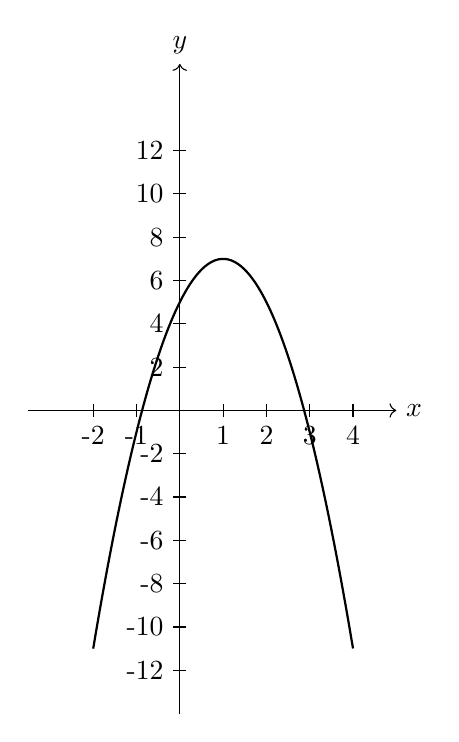
\begin{tikzpicture}[scale=0.55]
\draw[->] (-3.5,0) -- (5,0) node[right] {$x$};
\draw[->] (0,-7) -- (0,8) node[above] {$y$};
\foreach \x in {-2,-1,1,2,3,4}{
  \draw (\x,0.15) -- (\x,-0.15) node[below] {\x};
}
\foreach \y/\label in {-6/-12, -5/-10, -4/-8, -3/-6, -2/-4, -1/-2, 1/2, 2/4, 3/6, 4/8, 5/10, 6/12}{
  \draw (0.15,\y) -- (-0.15,\y) node[left] {\label};
}
\draw[thick,smooth,domain=-2:4,samples=80] plot (\x, {(5 + 4*\x - 2*\x*\x)/2});
\end{tikzpicture}
\end{center}

\begin{center}\itshape [Parabola of $f(x) = 5 + 4x - 2x^2$ --- see original paper for grid scale]\end{center}
\qmarks{5 marks}

\subhead{(c) (i) Draw an appropriate line on the graph and use it to estimate the solutions of $5 + 4x - 2x^2 = 3$.}

Solutions: $x = -0.4$ and $x = 2.4$ (from graph).
\qmarks{3 marks}

\hfill\textit{Total 12 marks}

\newpage
% ==========================================================
\begin{center}
\textbf{GEOMETRY AND TRIGONOMETRY}
\end{center}

\qhead{9. The diagram below shows quadrilaterals H, P and N. Quadrilaterals P and N are images of Quadrilateral H after two different transformations.}

\begin{center}
\fbox{\parbox{0.6\textwidth}{\centering\itshape [Quadrilateral grid with H, P, N --- see original paper]}}
\end{center}

\subhead{(a) Describe fully the single transformation that maps}

\textit{(i) Quadrilateral H onto Quadrilateral N.}

Quadrilateral H is mapped onto Quadrilateral N by a rotation of $90^{\circ}$ anticlockwise about the origin.
\qmarks{3 marks}

\textit{(ii) Quadrilateral H onto Quadrilateral P.}

Quadrilateral H is mapped onto Quadrilateral P by a translation using the vector $\begin{pmatrix} 2 \\ -5 \end{pmatrix}$.
\qmarks{2 marks}

\subhead{(b) On the grid, draw the image of Quadrilateral H after it undergoes the following transformations.}

\textit{(i) An enlargement with scale factor 2 about the centre $(0,-1)$. Label this image $M$.} (See grid.)
\qmarks{2 marks}

\textit{(ii) A reflection in the line $y = -x$. Label this image $L$.} (See grid.)
\qmarks{2 marks}

\subhead{(c) The diagram shows three pillars, L, M and N, on level ground. $MN = 12$ km and $LN = 15$ km. $L$ is due west of $N$. The bearing of $M$ from $N$ is $291^{\circ}$.}

\begin{center}
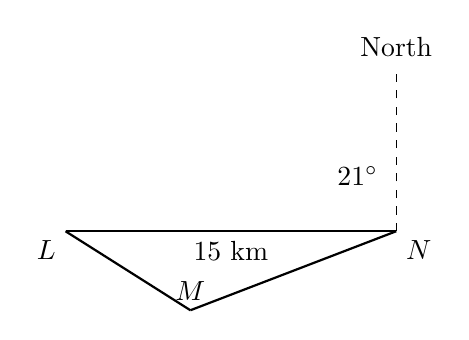
\begin{tikzpicture}[scale=0.7]
\coordinate (N) at (6,0);
\coordinate (L) at (0,0);
\coordinate (M) at ($(N) + (291-90:4)$);
\draw[thick] (L)--(N);
\draw[thick] (N)--(M);
\draw[thick] (L)--(M);
\draw[dashed] (N) -- ++(0,3) node[above] {North};
\node[below left] at (L) {$L$};
\node[below right] at (N) {$N$};
\node[above] at (M) {$M$};
\node[below] at (3,0) {$15$ km};
\node at (5.3,1.0) {$21^{\circ}$};
\end{tikzpicture}
\end{center}

Calculate:

\textit{(i) Angle $MNL$.}
\begin{align*}
\text{Bearing of } M \text{ from } N &= 291^{\circ} \\
\text{Bearing of } L \text{ from } N &= 270^{\circ} \\
\angle MNL &= 291^{\circ} - 270^{\circ} = 21^{\circ}
\end{align*}
\qmarks{1 mark}

\textit{(ii) The length of $LM$.}
\begin{align*}
a^2 &= b^2 + c^2 - 2bc\cos A \\
a^2 &= (15)^2 + (12)^2 - 2(15)(12)\cos(21^{\circ}) \\
a^2 &= 32.91 \\
a &= 5.74 \text{ km}
\end{align*}
\qmarks{2 marks}

\hfill\textit{Total 12 marks}

\newpage
% ==========================================================
\begin{center}
\textbf{VECTORS AND MATRICES}
\end{center}

\qhead{10. (a) The diagram below shows a scalene triangle, $OPQ$, with vectors $\vec{OP} = \mathbf{u}$ and $\vec{OQ} = 2\mathbf{v}$. The point $T$ is positioned on the line $PQ$ such that $PT:TQ = 3:2$.}

\begin{center}
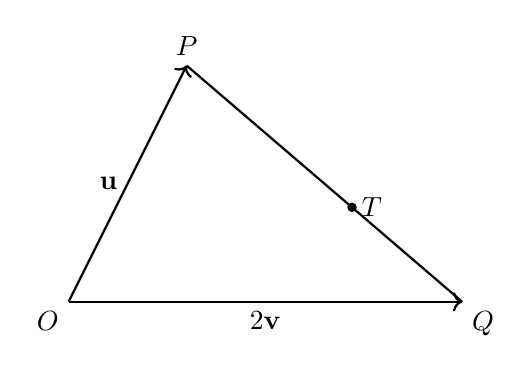
\begin{tikzpicture}[scale=1]
\coordinate (O) at (0,0);
\coordinate (P) at (1.5,3);
\coordinate (Q) at (5,0);
\coordinate (T) at ($(P)!3/5!(Q)$);
\draw[->,thick] (O)--(P) node[midway,left] {$\mathbf{u}$};
\draw[->,thick] (O)--(Q) node[midway,below] {$2\mathbf{v}$};
\draw[thick] (P)--(Q);
\filldraw (T) circle (1.5pt);
\node[above] at (P) {$P$};
\node[below left] at (O) {$O$};
\node[below right] at (Q) {$Q$};
\node[right] at (T) {$T$};
\end{tikzpicture}
\end{center}

Derive a simplified expression, in terms of $\mathbf{u}$ and $\mathbf{v}$, for

\subhead{(i) $\vec{PQ}$.}
\begin{align*}
\vec{PQ} &= \vec{PO} + \vec{OQ} \\
&= -\mathbf{u} + 2\mathbf{v} \\
&= 2\mathbf{v} - \mathbf{u}
\end{align*}
\qmarks{1 mark}

\subhead{(ii) $\vec{OT}$.}
\begin{align*}
\vec{OT} &= \vec{OP} + \tfrac{3}{5}\vec{PQ} \\
&= \mathbf{u} + \tfrac{3}{5}(2\mathbf{v} - \mathbf{u}) \\
&= \mathbf{u} + \tfrac{6}{5}\mathbf{v} - \tfrac{3}{5}\mathbf{u} \\
&= \tfrac{2}{5}\mathbf{u} + \tfrac{6}{5}\mathbf{v}
\end{align*}
\qmarks{2 marks}

\subhead{(b) (i) Write down the $2\times 2$ matrices that represent the following transformations.}

\textit{a) An enlargement with centre $(0,0)$ and a scale factor of 8.}
\[ \begin{pmatrix} 8 & 0 \\ 0 & 8 \end{pmatrix} \]

\textit{b) A reflection in the $x$-axis.}
\[ \begin{pmatrix} 1 & 0 \\ 0 & -1 \end{pmatrix} \]

\textit{c) An enlargement with centre $(0,0)$ and scale factor 8, followed by a reflection in the $x$-axis.}
\[ \begin{pmatrix} 1 & 0 \\ 0 & -1 \end{pmatrix}\begin{pmatrix} 8 & 0 \\ 0 & 8 \end{pmatrix} = \begin{pmatrix} 8 & 0 \\ 0 & -8 \end{pmatrix} \]
\qmarks{4 marks}

\subhead{(ii) The matrices $R$ and $Q$ are expressed in terms of the constants $k$ and $c$.}
\[ R = \begin{pmatrix} 6 & 1 \\ 4 & 2 \end{pmatrix}, \quad Q = \begin{pmatrix} k & 1 \\ c & -6 \end{pmatrix} \]

\textit{a) Calculate the matrix product $RQ$ in terms of $k$ and $c$.}
\begin{align*}
RQ &= \begin{pmatrix} 6 & 1 \\ 4 & 2 \end{pmatrix}\begin{pmatrix} k & 1 \\ c & -6 \end{pmatrix} \\
&= \begin{pmatrix} 6k + c & 6 - 6 \\ 4k + 2c & 4 - 12 \end{pmatrix} \\
&= \begin{pmatrix} 6k + c & 0 \\ 4k + 2c & -8 \end{pmatrix}
\end{align*}
\qmarks{2 marks}

\subhead{(iii) $RQ$ represents the transformation of an enlargement with centre $(0,0)$ and a scale factor of 8, followed by a reflection in the $x$-axis. Determine the values of $k$ and $c$.}
\[ \begin{pmatrix} 6k + c & 0 \\ 4k + 2c & -8 \end{pmatrix} = \begin{pmatrix} 8 & 0 \\ 0 & -8 \end{pmatrix} \]

Thus:
\begin{align*}
6k + c &= 8 \quad \text{Eq 1} \\
4k + 2c &= 0 \quad \text{Eq 2}
\end{align*}

Eq 1 $\times 2$: $12k + 2c = 16$ \quad (Eq 3)

Eq 3 $-$ Eq 2:
\begin{align*}
8k &= 16 \\
k &= 2
\end{align*}

Substitute into Eq 1:
\begin{align*}
6(2) + c &= 8 \\
c &= 8 - 12 \\
c &= -4
\end{align*}
\qmarks{3 marks}

\hfill\textit{Total 12 marks}

\vspace{2em}
\begin{center}
\textbf{END OF TEST}
\end{center}

\end{document}
